\documentclass{standalone}
\usepackage{tikz}
\usetikzlibrary{patterns, positioning}
\usepackage[sfdefault]{ClearSans} %% option 'sfdefault' activates Clear Sans as the default text font
\usepackage[T1]{fontenc}

\begin{document}
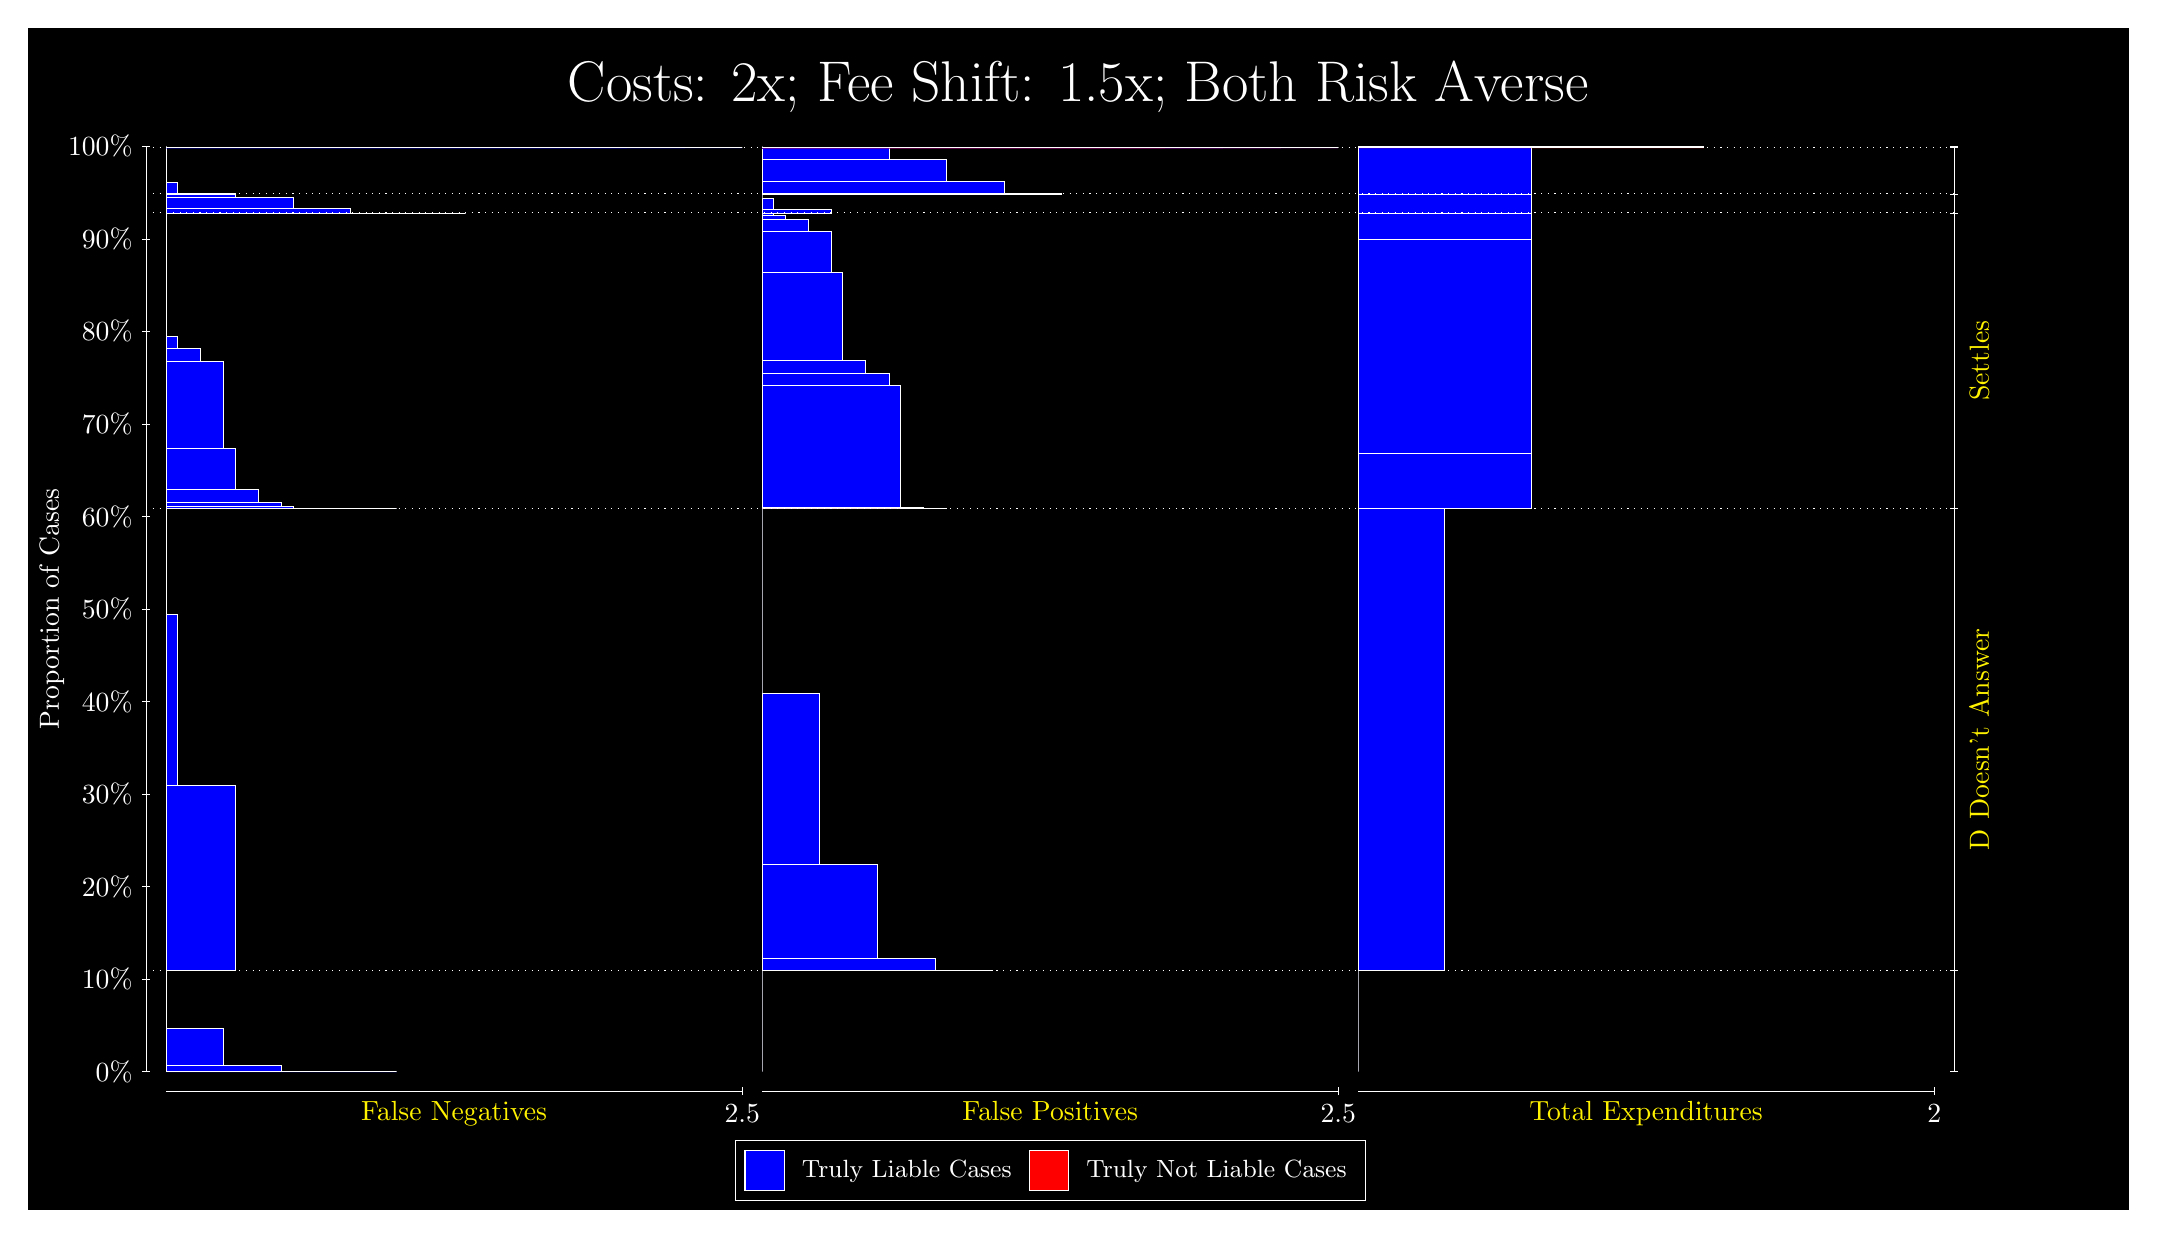
\begin{tikzpicture}
\draw[fill=black] (0,0) rectangle (26.667,15);
\draw[text=white] (0,13.5) rectangle (26.667,15) node[midway] {\huge Costs: 2x; Fee Shift: 1.5x; Both Risk Averse};
\draw[white, very thin] (1.5,1.75) -- (1.5,13.5);
\node[rotate=90, text=white, anchor=center] at (0.3, 7.625) {Proportion of Cases};
\draw[white, very thin] (1.45,1.75) -- (1.55,1.75);
\node[text=white, anchor=east] at (1.45, 1.75) {0\%};
\draw[white, very thin] (1.45,2.925) -- (1.55,2.925);
\node[text=white, anchor=east] at (1.45, 2.925) {10\%};
\draw[white, very thin] (1.45,4.1) -- (1.55,4.1);
\node[text=white, anchor=east] at (1.45, 4.1) {20\%};
\draw[white, very thin] (1.45,5.275) -- (1.55,5.275);
\node[text=white, anchor=east] at (1.45, 5.275) {30\%};
\draw[white, very thin] (1.45,6.45) -- (1.55,6.45);
\node[text=white, anchor=east] at (1.45, 6.45) {40\%};
\draw[white, very thin] (1.45,7.625) -- (1.55,7.625);
\node[text=white, anchor=east] at (1.45, 7.625) {50\%};
\draw[white, very thin] (1.45,8.8) -- (1.55,8.8);
\node[text=white, anchor=east] at (1.45, 8.8) {60\%};
\draw[white, very thin] (1.45,9.975) -- (1.55,9.975);
\node[text=white, anchor=east] at (1.45, 9.975) {70\%};
\draw[white, very thin] (1.45,11.15) -- (1.55,11.15);
\node[text=white, anchor=east] at (1.45, 11.15) {80\%};
\draw[white, very thin] (1.45,12.325) -- (1.55,12.325);
\node[text=white, anchor=east] at (1.45, 12.325) {90\%};
\draw[white, very thin] (1.45,13.5) -- (1.55,13.5);
\node[text=white, anchor=east] at (1.45, 13.5) {100\%};

\draw[white, very thin] (24.457,1.75) -- (24.457,13.5);
\draw[white, very thin] (24.407,1.75) -- (24.507,1.75);
\node[anchor=west] at (24.407, 1.75) {};
\draw[white, very thin] (24.407,3.0334) -- (24.507,3.0334);
\node[anchor=west] at (24.407, 3.0334) {};
\draw[white, very thin] (24.407,8.9016) -- (24.507,8.9016);
\node[anchor=west] at (24.407, 8.9016) {};
\draw[white, very thin] (24.407,12.655) -- (24.507,12.655);
\node[anchor=west] at (24.407, 12.655) {};
\draw[white, very thin] (24.407,12.897) -- (24.507,12.897);
\node[anchor=west] at (24.407, 12.897) {};
\draw[white, very thin] (24.407,13.485) -- (24.507,13.485);
\node[anchor=west] at (24.407, 13.485) {};
\draw[white, very thin] (24.407,13.5) -- (24.507,13.5);
\node[anchor=west] at (24.407, 13.5) {};

\draw[white, very thin, fill=blue] (1.75,1.75) rectangle (4.6775,1.75);
\draw[white, very thin, fill=blue] (1.75,1.75) rectangle (3.9457,1.7507);
\draw[white, very thin, fill=blue] (1.75,1.7507) rectangle (3.2138,1.8317);
\draw[white, very thin, fill=blue] (1.75,1.8317) rectangle (2.4819,2.3027);
\draw[white, very thin, fill=red] (1.75,2.3027) rectangle (1.75,2.3027);
\draw[white, very thin, fill=blue] (1.75,2.3027) rectangle (1.75,3.0334);
\draw[white, very thin, fill=blue] (1.75,3.0334) rectangle (2.6283,5.3815);
\draw[white, very thin, fill=blue] (1.75,5.3815) rectangle (1.8964,7.5564);
\draw[white, very thin, fill=red] (1.75,7.5564) rectangle (1.75,7.5564);
\draw[white, very thin, fill=blue] (1.75,7.5564) rectangle (1.75,8.9016);
\draw[white, very thin, fill=blue] (1.75,8.9016) rectangle (4.6775,8.9016);
\draw[white, very thin, fill=blue] (1.75,8.9016) rectangle (4.3848,8.9016);
\draw[white, very thin, fill=blue] (1.75,8.9016) rectangle (4.092,8.9016);
\draw[white, very thin, fill=blue] (1.75,8.9016) rectangle (3.9457,8.9016);
\draw[white, very thin, fill=blue] (1.75,8.9016) rectangle (3.6529,8.9051);
\draw[white, very thin, fill=blue] (1.75,8.9051) rectangle (3.3602,8.9289);
\draw[white, very thin, fill=blue] (1.75,8.9289) rectangle (3.2138,8.9826);
\draw[white, very thin, fill=blue] (1.75,8.9826) rectangle (2.921,9.1393);
\draw[white, very thin, fill=blue] (1.75,9.1393) rectangle (2.6283,9.6607);
\draw[white, very thin, fill=blue] (1.75,9.6607) rectangle (2.4819,10.774);
\draw[white, very thin, fill=blue] (1.75,10.774) rectangle (2.1891,10.938);
\draw[white, very thin, fill=blue] (1.75,10.938) rectangle (1.8964,11.091);
\draw[white, very thin, fill=red] (1.75,11.091) rectangle (1.75,11.091);
\draw[white, very thin, fill=blue] (1.75,11.091) rectangle (1.75,12.655);
\draw[white, very thin, fill=blue] (1.75,12.655) rectangle (5.5558,12.655);
\draw[white, very thin, fill=blue] (1.75,12.655) rectangle (4.8239,12.655);
\draw[white, very thin, fill=blue] (1.75,12.655) rectangle (4.092,12.716);
\draw[white, very thin, fill=blue] (1.75,12.716) rectangle (3.3602,12.852);
\draw[white, very thin, fill=blue] (1.75,12.852) rectangle (2.6283,12.897);
\draw[white, very thin, fill=red] (1.75,12.897) rectangle (1.75,12.897);
\draw[white, very thin, fill=blue] (1.75,12.897) rectangle (2.6283,12.899);
\draw[white, very thin, fill=blue] (1.75,12.899) rectangle (1.8964,13.045);
\draw[white, very thin, fill=red] (1.75,13.045) rectangle (1.75,13.045);
\draw[white, very thin, fill=blue] (1.75,13.045) rectangle (1.75,13.485);
\draw[white, very thin, fill=blue] (1.75,13.485) rectangle (9.0689,13.485);
\draw[white, very thin, fill=blue] (1.75,13.485) rectangle (8.337,13.485);
\draw[white, very thin, fill=blue] (1.75,13.485) rectangle (7.6051,13.485);
\draw[white, very thin, fill=blue] (1.75,13.485) rectangle (6.8732,13.488);
\draw[white, very thin, fill=blue] (1.75,13.488) rectangle (6.1413,13.491);
\draw[white, very thin, fill=blue] (1.75,13.491) rectangle (5.4094,13.491);
\draw[white, very thin, fill=blue] (1.75,13.491) rectangle (3.0674,13.491);
\draw[white, very thin, fill=blue] (1.75,13.491) rectangle (2.3355,13.491);
\draw[white, very thin, fill=red] (1.75,13.491) rectangle (1.75,13.491);
\draw[white, very thin, fill=blue] (1.75,13.491) rectangle (1.75,13.5);
\draw[white, very thin, fill=red] (9.3189,1.75) rectangle (9.3189,1.75);
\draw[white, very thin, fill=blue] (9.3189,1.75) rectangle (9.3189,3.0334);
\draw[white, very thin, fill=red] (9.3189,3.0334) rectangle (12.246,3.0334);
\draw[white, very thin, fill=blue] (9.3189,3.0334) rectangle (12.246,3.0347);
\draw[white, very thin, fill=blue] (9.3189,3.0347) rectangle (11.515,3.1907);
\draw[white, very thin, fill=blue] (9.3189,3.1907) rectangle (10.783,4.3785);
\draw[white, very thin, fill=blue] (9.3189,4.3785) rectangle (10.051,6.5534);
\draw[white, very thin, fill=blue] (9.3189,6.5534) rectangle (9.3189,8.9016);
\draw[white, very thin, fill=red] (9.3189,8.9016) rectangle (11.661,8.9016);
\draw[white, very thin, fill=blue] (9.3189,8.9016) rectangle (11.661,8.9058);
\draw[white, very thin, fill=red] (9.3189,8.9058) rectangle (11.368,8.9058);
\draw[white, very thin, fill=blue] (9.3189,8.9058) rectangle (11.368,8.9109);
\draw[white, very thin, fill=red] (9.3189,8.9109) rectangle (11.075,8.9109);
\draw[white, very thin, fill=blue] (9.3189,8.9109) rectangle (11.075,10.466);
\draw[white, very thin, fill=blue] (9.3189,10.466) rectangle (10.929,10.618);
\draw[white, very thin, fill=blue] (9.3189,10.618) rectangle (10.636,10.783);
\draw[white, very thin, fill=blue] (9.3189,10.783) rectangle (10.344,11.896);
\draw[white, very thin, fill=blue] (9.3189,11.896) rectangle (10.197,12.417);
\draw[white, very thin, fill=blue] (9.3189,12.417) rectangle (9.9044,12.574);
\draw[white, very thin, fill=blue] (9.3189,12.574) rectangle (9.6116,12.628);
\draw[white, very thin, fill=blue] (9.3189,12.628) rectangle (9.4652,12.651);
\draw[white, very thin, fill=blue] (9.3189,12.651) rectangle (9.3189,12.655);
\draw[white, very thin, fill=red] (9.3189,12.655) rectangle (10.197,12.655);
\draw[white, very thin, fill=blue] (9.3189,12.655) rectangle (10.197,12.7);
\draw[white, very thin, fill=blue] (9.3189,12.7) rectangle (9.4652,12.836);
\draw[white, very thin, fill=blue] (9.3189,12.836) rectangle (9.3189,12.897);
\draw[white, very thin, fill=red] (9.3189,12.897) rectangle (13.125,12.897);
\draw[white, very thin, fill=blue] (9.3189,12.897) rectangle (13.125,12.905);
\draw[white, very thin, fill=blue] (9.3189,12.905) rectangle (12.393,13.057);
\draw[white, very thin, fill=blue] (9.3189,13.057) rectangle (11.661,13.336);
\draw[white, very thin, fill=blue] (9.3189,13.336) rectangle (10.929,13.483);
\draw[white, very thin, fill=blue] (9.3189,13.483) rectangle (10.197,13.485);
\draw[white, very thin, fill=red] (9.3189,13.485) rectangle (16.638,13.485);
\draw[white, very thin, fill=blue] (9.3189,13.485) rectangle (16.638,13.485);
\draw[white, very thin, fill=red] (9.3189,13.485) rectangle (15.906,13.485);
\draw[white, very thin, fill=blue] (9.3189,13.485) rectangle (15.906,13.485);
\draw[white, very thin, fill=red] (9.3189,13.485) rectangle (15.174,13.485);
\draw[white, very thin, fill=blue] (9.3189,13.485) rectangle (15.174,13.485);
\draw[white, very thin, fill=red] (9.3189,13.485) rectangle (14.442,13.485);
\draw[white, very thin, fill=blue] (9.3189,13.485) rectangle (14.442,13.488);
\draw[white, very thin, fill=blue] (9.3189,13.488) rectangle (13.71,13.493);
\draw[white, very thin, fill=blue] (9.3189,13.493) rectangle (12.978,13.493);
\draw[white, very thin, fill=blue] (9.3189,13.493) rectangle (12.246,13.493);
\draw[white, very thin, fill=blue] (9.3189,13.493) rectangle (11.515,13.493);
\draw[white, very thin, fill=red] (9.3189,13.493) rectangle (9.3189,13.493);
\draw[white, very thin, fill=blue] (9.3189,13.493) rectangle (9.3189,13.5);
\draw[white, very thin, fill=red] (16.888,1.75) rectangle (16.888,1.75);
\draw[white, very thin, fill=blue] (16.888,1.75) rectangle (16.888,3.0334);
\draw[white, very thin, fill=red] (16.888,3.0334) rectangle (17.986,3.0334);
\draw[white, very thin, fill=blue] (16.888,3.0334) rectangle (17.986,8.9016);
\draw[white, very thin, fill=red] (16.888,8.9016) rectangle (19.083,8.9016);
\draw[white, very thin, fill=blue] (16.888,8.9016) rectangle (19.083,9.6037);
\draw[white, very thin, fill=red] (16.888,9.6037) rectangle (19.083,9.6037);
\draw[white, very thin, fill=blue] (16.888,9.6037) rectangle (19.083,12.325);
\draw[white, very thin, fill=red] (16.888,12.325) rectangle (19.083,12.325);
\draw[white, very thin, fill=blue] (16.888,12.325) rectangle (19.083,12.655);
\draw[white, very thin, fill=red] (16.888,12.655) rectangle (19.083,12.655);
\draw[white, very thin, fill=blue] (16.888,12.655) rectangle (19.083,12.897);
\draw[white, very thin, fill=red] (16.888,12.897) rectangle (19.083,12.897);
\draw[white, very thin, fill=blue] (16.888,12.897) rectangle (19.083,13.485);
\draw[white, very thin, fill=red] (16.888,13.485) rectangle (21.279,13.485);
\draw[white, very thin, fill=blue] (16.888,13.485) rectangle (21.279,13.5);
\draw[white, dotted] (1.5,3.0334) -- (24.457,3.0334);
\draw[white, dotted] (1.5,8.9016) -- (24.457,8.9016);
\draw[white, dotted] (1.5,12.655) -- (24.457,12.655);
\draw[white, dotted] (1.5,12.897) -- (24.457,12.897);
\draw[white, dotted] (1.5,13.485) -- (24.457,13.485);
\draw[white, very thin] (1.75,1.5) -- (9.0689,1.5);
\node[text=yellow, anchor=north] at (5.4094, 1.5) {False Negatives};
\draw[white, very thin] (9.0689,1.45) -- (9.0689,1.55);
\node[text=white, anchor=north] at (9.0689, 1.45) {2.5};

\draw[white, very thin] (9.3189,1.5) -- (16.638,1.5);
\node[text=yellow, anchor=north] at (12.978, 1.5) {False Positives};
\draw[white, very thin] (16.638,1.45) -- (16.638,1.55);
\node[text=white, anchor=north] at (16.638, 1.45) {2.5};

\draw[white, very thin] (16.888,1.5) -- (24.207,1.5);
\node[text=yellow, anchor=north] at (20.547, 1.5) {Total Expenditures};
\draw[white, very thin] (24.207,1.45) -- (24.207,1.55);
\node[text=white, anchor=north] at (24.207, 1.45) {2};


\node[text=yellow, centered, rotate=90] at (24.777, 5.9675) {D Doesn't Answer};
\node[text=yellow, centered, rotate=90] at (24.777, 10.778) {Settles};




\draw (12.978300999999998,1.5) node[draw=none] (baseCoordinate) {};
\begin{scope}[align=center]
        \matrix[scale=0.5, draw=white, below=0.5cm of baseCoordinate, nodes={draw}, column sep=0.1cm]{
            \node[rectangle, draw, minimum width=0.5cm, minimum height=0.5cm, fill=blue] {}; &
            \node[draw=none, font=\small, text=white] (B) {Truly Liable Cases}; &
            \node[rectangle, draw, minimum width=0.5cm, minimum height=0.5cm, fill=red] {}; &
            \node[draw=none, font=\small, text=white] (B) {Truly Not Liable Cases}; \\
            };
\end{scope}

\end{tikzpicture}
\end{document}